% =====================================================================
% Section 6: Experiments (sec:exp).
% Floats, in numbering order: Table 3 (tables/tab_main.tex, table*),
% Fig. 4 (fig:ql, single column, Sec. 6.2), Fig. 5 (fig:gap, figure*,
% defined at the start of Sec. 6.3 so that it lands near Sec. 6.4),
% Table 4 (tables/tab_factorial.tex) and Table 5 (tables/tab_aux.tex),
% both input in Sec. 6.3 so that Table 5 is not pushed past Sec. 7,
% and Table 6 (tables/tab_ablation.tex).
% Measured so far (preliminary, \prelim): the offline rows of Table 3 and
% the two ASR WERs of Table 5. Everything else is pending: the result
% paragraphs are templates with \tbdtext; do not add findings before the
% runs exist.
% Wording: the offline systems and Gold->LLM (MU2) get oracle input but are
% not called bounds (no dialogue history; Whisper ST already passes
% Gold->LLM on De->En BLEU). R and Fig. 5 use one pipeline under both
% wrappers, that of Table 4.
% =====================================================================
\section{Experiments}\label{sec:exp}

% =====================================================================
% Table 3 (tab:main): main results on CST-Bench-TAXI, L0 natural timing,
% ideal clock (table*, 8pt; 529pt wide at 9pt, 480pt at 8pt). Included at the start of Sec. 6.
% Measured so far (preliminary, \prelim): BLEU, chrF and StreamLAAL of the
% three offline rows; their EndOffset is 0 by construction on the ideal
% clock. They were scored with gold turn IDs (scorer oracle mode, no
% resegmentation); the caption says so. Every other cell is pending
% (\tbd = blank); -- marks a direction the system does not cover, and the
% pooled columns of single-direction systems. Systems are defined in Sec. 6.1
% (sec:exp-setup); names follow Table A5 (tab:conditions), and the caption
% of Fig. 4 (fig:ql) maps its legend labels to them.
% =====================================================================
\begin{table*}[t]
  \caption{Real dialogues: \taxi, L0 natural timing, ideal clock. Rows: upper bounds with oracle input, the consecutive cascade, streaming systems and \model (\cref{sec:exp-setup}; LLM: Qwen3.8-27B), each at its main operating point; \model M2 commits translations at turn ends, and M3 at MU2 units with a low or a high $\delta_t$. Seg.: oracle = gold turns and source language; realistic = VAD and language-ID routing; none = the system segments the stream itself. Per direction: mean \laal and median \eo in seconds; the last three columns pool both directions (switch latency: median, in seconds) and do not apply to single-direction systems, which cannot be the best pipeline (\cref{tab:factorial,fig:gap}). \Cref{tab:conditions} gives 95\% session-bootstrap CIs for the rows it repeats, except for BLEU. Blank: pending; --: direction not covered. $^\dagger$preliminary and scored by gold turn ID (oracle mode of \cref{app:scorer}), not resegmented; to be re-run under the final protocol. $^\ddagger$0 by construction: the output is emitted at the oracle turn end.}
  \label{tab:main}
  \centering
  \fontsize{8}{9.5}\selectfont % 8pt (ICML \footnotesize is 9pt): fits the width
  \setlength{\tabcolsep}{2.5pt}
  \begin{tabular}{@{}ll*{13}{c}@{}}
    \toprule
    & & \multicolumn{5}{c}{\ende} & \multicolumn{5}{c}{\deen} & \multicolumn{3}{c}{Both directions} \\
    \cmidrule(lr){3-7}\cmidrule(lr){8-12}\cmidrule(l){13-15}
    System & Seg.
      & COMET & BLEU & chrF & \makecell[b]{Stream-\\LAAL} & \makecell[b]{End-\\Offset}
      & COMET & BLEU & chrF & \makecell[b]{Stream-\\LAAL} & \makecell[b]{End-\\Offset}
      & \makecell[b]{Wrong\\dir.\ (\%)} & \makecell[b]{Switch\\latency} & \makecell[b]{Empty\\turns (\%)} \\
    \midrule
    Gold$\to$LLM & oracle
      & \tbd & \prelim{48.31} & \prelim{71.72} & \prelim{4.62} & $0^{\ddagger}$
      & \tbd & \prelim{30.60} & \prelim{58.05} & \prelim{3.09} & $0^{\ddagger}$
      & \tbd & \tbd & \tbd \\
    ASR$\to$LLM & oracle
      & \tbd & \prelim{42.66} & \prelim{67.97} & \prelim{4.62} & $0^{\ddagger}$
      & \tbd & \prelim{28.11} & \prelim{56.61} & \prelim{3.09} & $0^{\ddagger}$
      & \tbd & \tbd & \tbd \\
    Whisper ST & oracle
      & --   & --   & --   & --   & --
      & \tbd & \prelim{30.69} & \prelim{56.67} & \prelim{3.09} & $0^{\ddagger}$
      & --   & --   & --   \\
    Gold$\to$LLM (MU2) & oracle
      & \tbd & \tbd & \tbd & \tbd & \tbd
      & \tbd & \tbd & \tbd & \tbd & \tbd
      & \tbd & \tbd & \tbd \\
    \midrule
    Consecutive cascade & realistic
      & \tbd & \tbd & \tbd & \tbd & \tbd
      & \tbd & \tbd & \tbd & \tbd & \tbd
      & \tbd & \tbd & \tbd \\
    \midrule
    \multirow{2}{*}{SeamlessStreaming} & oracle
      & \tbd & \tbd & \tbd & \tbd & \tbd
      & \tbd & \tbd & \tbd & \tbd & \tbd
      & \tbd & \tbd & \tbd \\
      & realistic
      & \tbd & \tbd & \tbd & \tbd & \tbd
      & \tbd & \tbd & \tbd & \tbd & \tbd
      & \tbd & \tbd & \tbd \\
    2$\times$SeamlessStreaming & none
      & \tbd & \tbd & \tbd & \tbd & \tbd
      & \tbd & \tbd & \tbd & \tbd & \tbd
      & \tbd & \tbd & \tbd \\
    \multirow{2}{*}{Streaming cascade} & oracle
      & \tbd & \tbd & \tbd & \tbd & \tbd
      & \tbd & \tbd & \tbd & \tbd & \tbd
      & \tbd & \tbd & \tbd \\
      & realistic
      & \tbd & \tbd & \tbd & \tbd & \tbd
      & \tbd & \tbd & \tbd & \tbd & \tbd
      & \tbd & \tbd & \tbd \\
    \multirow{2}{*}{M4T v2 + AlignAtt} & oracle
      & \tbd & \tbd & \tbd & \tbd & \tbd
      & \tbd & \tbd & \tbd & \tbd & \tbd
      & \tbd & \tbd & \tbd \\
      & realistic
      & \tbd & \tbd & \tbd & \tbd & \tbd
      & \tbd & \tbd & \tbd & \tbd & \tbd
      & \tbd & \tbd & \tbd \\
    \multirow{2}{*}{StreamSpeech} & oracle
      & --   & --   & --   & --   & --
      & \tbd & \tbd & \tbd & \tbd & \tbd
      & --   & --   & --   \\
      & realistic
      & --   & --   & --   & --   & --
      & \tbd & \tbd & \tbd & \tbd & \tbd
      & --   & --   & --   \\
    \multirow{2}{*}{InfiniSST} & oracle
      & \tbd & \tbd & \tbd & \tbd & \tbd
      & --   & --   & --   & --   & --
      & --   & --   & --   \\
      & realistic
      & \tbd & \tbd & \tbd & \tbd & \tbd
      & --   & --   & --   & --   & --
      & --   & --   & --   \\
    \midrule
    \model M2 & none
      & \tbd & \tbd & \tbd & \tbd & \tbd
      & \tbd & \tbd & \tbd & \tbd & \tbd
      & \tbd & \tbd & \tbd \\
    \model M3, low $\delta_t$ & none
      & \tbd & \tbd & \tbd & \tbd & \tbd
      & \tbd & \tbd & \tbd & \tbd & \tbd
      & \tbd & \tbd & \tbd \\
    \model M3, high $\delta_t$ & none
      & \tbd & \tbd & \tbd & \tbd & \tbd
      & \tbd & \tbd & \tbd & \tbd & \tbd
      & \tbd & \tbd & \tbd \\
    \bottomrule
  \end{tabular}
\end{table*}


We answer RQ1--RQ4 (\cref{sec:intro}) on real dialogues first; synthetic sessions add the distant pair and a check against real rankings. Every comparison carries a session-clustered 95\% confidence interval (CI; \cref{app:repro}), and we do not interpret differences inside it.
\draftnote{planned: apart from the preliminary offline rows of \cref{tab:main} and ASR WERs of \cref{tab:aux}, no experiment of this section has been run}

\subsection{Setup}\label{sec:exp-setup}

\paragraph{Systems.}
Every system receives the session's language pair.
Offline systems cut each oracle turn from the mix and translate it after the turn ends, one turn per prompt and without dialogue history: Qwen3.8-27B (``LLM'') translates the gold transcript (Gold$\to$LLM) or the transcript of Qwen3-ASR-1.7B, given the language \citep[ASR$\to$LLM;][]{shi2026qwen3asr}, and Whisper-large-v3 translates speech into English \citep[Whisper ST;][]{radford2023robust}.
Gold$\to$LLM (MU2) is a streaming variant with oracle input: the LLM reads gold transcripts at forced-aligned word times and commits at the verified meaning units (MU2) of \cref{sec:model}, whose boundaries are found with the whole turn in view (non-causal).
The consecutive cascade detects turn ends with the realistic wrapper described below, then transcribes and translates each segment like ASR$\to$LLM.
The streaming systems are SeamlessStreaming \citep{seamless2023seamless}, StreamSpeech \citep{zhang2024streamspeech} (\deen only), InfiniSST \citep{ouyang2025infinisst} (\ende only) and two systems that run offline translation models with a streaming policy.
In the streaming cascade, the LLM re-translates the growing transcript of the Nemotron~3.5 streaming RNN-T \citep{nvidia2026nemotron35asr} and commits the prefix on which two consecutive outputs agree (LocalAgreement-2, LA-2; \citealp{liu2020lowlatency,polak2022cuni,machacek2023turning}).
M4T v2 + AlignAtt runs SeamlessM4T~v2 \citep{seamless2025joint,seamless2023seamless} with the AlignAtt policy \citep{papi2023alignatt} in simulstream \citep{gaido2025simulstream}.
As a naive bidirectional baseline, 2$\times$SeamlessStreaming runs one instance per target language on the whole mix, without routing.
\model runs as M2, which commits translations at turn ends, and as M3, which commits at MU2 units and runs at a low and a high $\delta_t$ (\cref{sec:model}).
\Cref{tab:baselines} lists checkpoints, sizes and licences.
\draftnote{InfiniSST only if its weights are released; Canary-1B-v2 \citep{sekoyan2025canary} with AlignAtt is optional; Hibiki-Zero (\deen; public weights) is not yet in the plan}

\paragraph{Wrappers and operating points.}
A system that translates one direction runs as one instance per target language behind a wrapper; we call the combination a pipeline (\cref{app:baselines}).
The oracle wrapper cuts gold turns from the mix and routes each by its gold source language.
The realistic wrapper segments the stream with Silero VAD \citep{silero2024silero} and routes each segment by spoken language identification restricted to the pair, decided at the segment start and re-routed if the decision flips.
Baselines are not fine-tuned.
Each streaming system has two operating points, one of them its main point, chosen once on the \syn calibration split by a rule fixed before any test run.
\draftnote{until \syn exists, documented defaults stand in for calibrated operating points; which of the two latency budgets gives the main point is still to be fixed}

\paragraph{Metrics and statistics.}
Per direction, we report COMET, chrF and BLEU, \laal (lag within a turn) and median \eo (the listener's wait after a turn); pooled over directions, we report wrong-direction words, median switch latency and empty turns (\cref{sec:bench}).
We rank systems by COMET rather than BLEU \citep{kocmi2021ship}; on \taxi, whose references are lowercase and unpunctuated, chrF takes its place if the two rank systems differently (\cref{sec:exp-validity}).
Latency uses the ideal clock; computation-aware latency, measured for one unbatched stream on one GPU type, is in \cref{tab:ca-latency}.
The oracle-gap recovery of \model is $R=(Q_{\mathrm{ours}}-Q_{\mathrm{real}})/(Q_{\mathrm{oracle}}-Q_{\mathrm{real}})$, where $Q$ is COMET: of \model, and of the pipeline of \cref{tab:factorial} under the oracle and the realistic wrapper; $R$ comes with a bootstrap CI and is reported only where the CI of the gap excludes 0.
Daggers mark preliminary numbers, to be re-run under the final protocol.

\subsection{Real dialogues (RQ1, RQ3)}\label{sec:exp-real}

\begin{figure}[t]
  \centering
  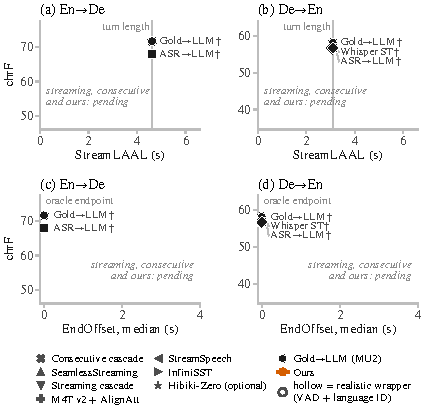
\includegraphics[width=0.89\columnwidth]{figures/fig4_quality_latency.pdf}
  \caption{Quality vs.\ latency on \taxi (L0 natural, ideal clock), per direction: chrF against \laal (a, b) and against median \eo (c, d). Black outlines mark systems with oracle input, although drawn hollow; by construction, the labelled offline systems sit at the mean source-turn duration on \laal (`turn length') and at 0 on \eo (`oracle endpoint'). The other systems are pending: filled markers will show oracle segmentation and hollow markers VAD and language-ID routing, with grey arrows joining the two for each system, and a vermillion curve will trace \model over its $\delta_t$ operating points. Legend: Seamless = SeamlessStreaming, Cascade-LA = streaming cascade, M4Tv2-AA = M4T v2 + AlignAtt, Ours = \model. chrF stands in until COMET is in the scorer. $^\dagger$preliminary; to be re-run under the final protocol.}
  \label{fig:ql}
\end{figure}

\Cref{tab:main} and \cref{fig:ql} compare all systems on \taxi under L0 natural timing.
Given oracle turns, Gold$\to$LLM reaches \prelim{48.31} BLEU and \prelim{71.72} chrF for \ende, and \prelim{30.60} and \prelim{58.05} for \deen.
ASR transcripts cost \prelim{5.65} and \prelim{2.49} BLEU, in line with the higher WER of Qwen3-ASR-1.7B on English than on German turns (\prelim{13.78}\% vs.\ \prelim{7.33}\%; \cref{tab:aux}), and Whisper ST reaches \prelim{30.69} BLEU into English.
These offline systems look instantaneous on \eo, at most about \prelim{0.2}\,s even with measured, batched computation (\cref{tab:ca-latency}), only because they receive oracle endpoints.
The consecutive cascade, which must detect endpoints, makes listeners wait a median of \tbdtext{}\,s at \tbdtext{} COMET.
Realistic segmentation costs the streaming systems \tbdtext{} COMET (arrows in \cref{fig:ql}), and \model reaches \tbdtext{} COMET at a median \eo of \tbdtext{}\,s without oracle input.

\subsection{Where pipelines fail (RQ1)}\label{sec:exp-fail}

% Fig. 5 is discussed in Sec. 6.4; it is defined here so that the full-width
% float can reach the top of the page that holds Sec. 6.4.
\begin{figure*}[t]
  \centering
  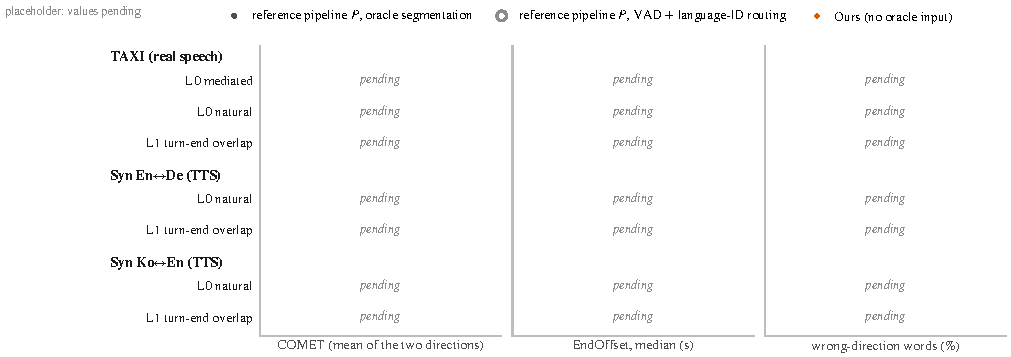
\includegraphics[width=\textwidth]{figures/fig5_oracle_gap.pdf}
  \caption{Where the conversational difficulty lies (values pending; numbers will be in \cref{tab:conditions}). For each timing condition and language pair: the best pipeline with oracle turn segmentation (filled) and with VAD and language-ID routing (hollow), and \model (diamond; no oracle input). One pipeline serves every row and both wrappers: that of \cref{tab:factorial}, with the highest realistic-wrapper COMET on \taxi L0 natural among pipelines that cover both directions, at its main operating point. Panels: COMET (mean of the two directions), median \eo and wrong-direction words.}
  \label{fig:gap}
\end{figure*}

% Table 5 (tab:aux) is input here, right after Table 4, so that it can
% share a page with Table 4 instead of floating past Sec. 7.
% =====================================================================
% Table 4 (tab:factorial): oracle-component factorial for the reference
% pipeline P of Sec. 6.1 on CST-Bench-TAXI, ideal clock (single column,
% 8pt). Included in Sec. 6.3.
% No values yet: every cell is pending (\tbd = blank); -- marks cells that
% do not apply. Language-ID routing accuracy is reported in the text; the
% factor effects E_T, E_L and their interaction, with their CIs, are
% defined in App. E, and the same factorial for the second-best pipeline
% goes to App. E. Cells carry no CIs; the caption points to App. E, not to
% tab:conditions, which has neither rows 2, 3, 5 nor the direction mean.
% How a VAD segment gets its gold language (the most-overlapping turn) is
% stated in App. D (app:baselines), not in the caption.
% =====================================================================
\begin{table}[t]
  \caption{Oracle-component factorial for the reference pipeline $P$ (\cref{sec:exp-setup}) on \taxi, ideal clock; factor effects with CIs: \cref{app:results}. \cmark: oracle T (gold turns, else VAD), L (gold language, else language ID; \cref{app:baselines}) or S (two-channel separation; L1 only). Row~4 is realistic. COMET: mean of both directions; $\Delta$COMET: L1 COMET minus row~1's L1 COMET.}
  \label{tab:factorial}
  \centering
  \fontsize{8}{9.5}\selectfont % 8pt (ICML \footnotesize is 9pt): fits the width
  \setlength{\tabcolsep}{2pt}
  \begin{tabular}{@{}cccccccccc@{}}
    \toprule
    & \multicolumn{3}{c}{Oracle} & \multicolumn{2}{c}{L0 natural} & \multicolumn{4}{c}{L1 turn-end overlap} \\
    \cmidrule(lr){2-4}\cmidrule(lr){5-6}\cmidrule(l){7-10}
    \# & T & L & S
      & COMET & \makecell[b]{Wrong\\dir.\ (\%)}
      & COMET & \makecell[b]{Wrong\\dir.\ (\%)} & \makecell[b]{Switch\\latency} & $\Delta$COMET \\
    \midrule
    1 & \cmark & \cmark & \xmark & \tbd & \tbd & \tbd & \tbd & \tbd & --   \\
    2 & \cmark & \xmark & \xmark & \tbd & \tbd & \tbd & \tbd & \tbd & \tbd \\
    3 & \xmark & \cmark & \xmark & \tbd & \tbd & \tbd & \tbd & \tbd & \tbd \\
    4 & \xmark & \xmark & \xmark & \tbd & \tbd & \tbd & \tbd & \tbd & \tbd \\
    5 & \cmark & \cmark & \cmark & --   & --   & \tbd & \tbd & \tbd & \tbd \\
    \midrule
    \multicolumn{4}{@{}l}{6\enspace\model} & \tbd & \tbd & \tbd & \tbd & \tbd & \tbd \\
    \bottomrule
  \end{tabular}
\end{table}

% =====================================================================
% Table 5 (tab:aux): transcription and two-speaker attribution
% (single column, \footnotesize). Included in Sec. 6.3, discussed in 6.5.
% Layout: systems as columns, set x metric as rows (fits one column; about
% 232pt in a 234.9pt column, so no eighth column fits).
% Measured so far (preliminary, \prelim): the two TAXI WERs of Qwen3-ASR-1.7B
% on oracle turns. Every other cell is pending (\tbd = blank); -- marks
% cells that do not apply (oracle speakers, offline output). The diarization
% baselines are called "diar." here so that they are not confused with the
% translation "streaming cascade" of Table 3. Context delays of the earlier
% single-speaker 0.6B backbones are in App. F, not here; tcpWER and DER
% without a collar are in App. E.
% =====================================================================
\begin{table}[t]
  \caption{Who said what: error rates (\%); systems: \cref{sec:exp-aux}. L0: L0 natural; Syn: \syn \pair{Ko}{En}. DER: 0.25\,s collar. Delay: median delay of transcript words. --: not applicable. $^\dagger$Preliminary.}
  \label{tab:aux}
  \centering
  \footnotesize
  \setlength{\tabcolsep}{2.6pt}
  \begin{tabular}{@{}llccccc@{}}
    \toprule
    & & & & & \multicolumn{2}{c}{\model} \\
    \cmidrule(l){6-7}
    Set & Metric & \makecell[b]{Oracle\\ASR} & \makecell[b]{Offline\\diar.} & \makecell[b]{Streaming\\diar.} & $\delta_s{=}2$ & $\delta_s{=}4$ \\
    \midrule
    \multirow{5}{*}{TAXI L0} & WER En     & \prelim{13.78} & \tbd & \tbd & \tbd & \tbd \\
                             & WER De     & \prelim{7.33}  & \tbd & \tbd & \tbd & \tbd \\
                             & cpWER      & \tbd & \tbd & \tbd & \tbd & \tbd \\
                             & DER        & --   & \tbd & \tbd & \tbd & \tbd \\
                             & Delay (ms) & --   & --   & \tbd & \tbd & \tbd \\
    \midrule
    \multirow{2}{*}{TAXI L1} & cpWER      & \tbd & \tbd & \tbd & \tbd & \tbd \\
                             & DER        & --   & \tbd & \tbd & \tbd & \tbd \\
    \midrule
    Syn L1                   & cpCER      & \tbd & \tbd & \tbd & \tbd & \tbd \\
    \bottomrule
  \end{tabular}
\end{table}


\Cref{tab:factorial} replaces one oracle component at a time for the best pipeline of \cref{tab:main}; \cref{app:results} repeats this for the second best.
We expect silence-based segmentation to merge turns across speaker changes: a 500\,ms threshold captures only 18--30\% of between-speaker intervals in conversational corpora \citep{heldner2010pauses}, and the median speaker-change gap of \taxi L0 natural is 0.223\,s.
Under L0 natural, turn segmentation costs \tbdtext{} COMET and routing \tbdtext{}, at \tbdtext{}\% language-ID routing accuracy; under L1, oracle separation recovers \tbdtext{} COMET.
Short turns are a further risk, as 59 \taxi turns have at most three words; \cref{app:results} breaks errors down by type (\cref{tab:failures}) and listener wait by source-turn duration (\cref{fig:turn-length}).

\subsection{Timing conditions and language pairs (RQ2, RQ3)}\label{sec:exp-timing}

\Cref{fig:gap} contrasts, for each timing condition and language pair, the best pipeline under both wrappers with \model.
On \taxi, the oracle--realistic COMET gap is \tbdtext{} under L0 mediated, \tbdtext{} under L0 natural and \tbdtext{} under L1, and \model recovers \tbdtext{}\% of it under L1.
Re-rendering \taxi with one fixed gap from $-0.6$ to 2\,s at every speaker change traces the dose--response (\cref{fig:gap-sweep}).
We compare language pairs only through each pair's gap to its own oracle, never through absolute scores.
The text-level unit pilot already shows a direction asymmetry in the distant pair: only 21\% of candidate commit points pass verification for \enko, against 54\% for \koen (\cref{app:units}).

\subsection{Who said what: transcripts and speakers}\label{sec:exp-aux}

\Cref{tab:aux} scores transcripts and speaker attribution with WER per language, cpWER \citep{watanabe2020chime} and DER.
The baselines are Qwen3-ASR-1.7B on oracle turns, an offline cascade of pyannote diarization \citep{bredin2023pyannote} and Qwen3-ASR-1.7B, and a streaming cascade of Streaming Sortformer \citep{park2025sortformer,medennikov2025streaming} and the Nemotron~3.5 streaming RNN-T.
\model reaches \tbdtext{}\% cpWER and \tbdtext{}\% DER on \taxi L1 at $\delta_s=2$.
DER needs care here: in the first release each speaker keeps one language, so the language reveals the speaker, and DER mostly measures boundary timing under short gaps and overlap; speakers who switch languages, which we exclude, would break this equivalence.

\subsection{Ablations: does the unified design help?}\label{sec:exp-ablation}

% =====================================================================
% Table 6 (tab:ablation): ablations of the model, one change per row
% (single column, 8pt). Included in Sec. 6.6.
% No values yet: every cell is pending (\tbd = blank).
% Rows marked ^\circ are optional runs; if a run is cut, delete its row
% rather than leaving it blank. Both COMET columns (L0 natural and L1) will
% hold "En->De / De->En" pairs, e.g. x\,/\,y; with COMET x100 and one
% decimal the filled table is 233.6pt wide in a 234.9pt column, so an eighth
% column does not fit (EndOffset under L1: 256.6pt; the model's is in
% tab:conditions). cpWER of the model is in tab:aux, not here.
% =====================================================================
\begin{table}[t]
  \caption{Ablations of \model, one change per row from the same M1 checkpoint. \model (M3) commits at MU2 units, uses speaker tags and sees L1 sessions in training; the next rows commit at turn ends instead (M2), keep only target-language tags, drop the L1 sessions, or train fixed-$\delta_t$ models instead of conditioning on $\delta_t$. M1$\to$LLM: same-backbone cascade (M1 transcripts, Qwen3.8-27B, LA-2); ASR$\to$1.7B LLM: size-matched cascade (Qwen3-ASR-1.7B, an LLM of about 1.7B parameters, LA-2). COMET is given as \ende\,/\,\deen; \laal is the mean over both directions and \eo and switch latency are medians, all in seconds; wrong-direction words in \%. All cells are pending. $^\circ$Optional run.}
  \label{tab:ablation}
  \centering
  \fontsize{8}{9.5}\selectfont % 8pt (ICML \footnotesize is 9pt): fits the width
  \setlength{\tabcolsep}{1.6pt}
  \begin{tabular}{@{}lcccccc@{}}
    \toprule
    & \multicolumn{3}{c}{L0 natural} & \multicolumn{3}{c}{L1 turn-end overlap} \\
    \cmidrule(lr){2-4}\cmidrule(l){5-7}
    Variant & COMET & \makecell[b]{Stream-\\LAAL} & \makecell[b]{End-\\Offset}
            & COMET & \makecell[b]{Wrong\\dir.} & \makecell[b]{Switch\\latency} \\
    \midrule
    \model (M3)                     & \tbd & \tbd & \tbd & \tbd & \tbd & \tbd \\
    \midrule
    turn-end commits                & \tbd & \tbd & \tbd & \tbd & \tbd & \tbd \\
    no speaker tags                 & \tbd & \tbd & \tbd & \tbd & \tbd & \tbd \\
    no L1 in training$^\circ$       & \tbd & \tbd & \tbd & \tbd & \tbd & \tbd \\
    fixed-$\delta_t$ models$^\circ$ & \tbd & \tbd & \tbd & \tbd & \tbd & \tbd \\
    \midrule
    M1$\to$LLM                      & \tbd & \tbd & \tbd & \tbd & \tbd & \tbd \\
    ASR$\to$1.7B LLM                & \tbd & \tbd & \tbd & \tbd & \tbd & \tbd \\
    \bottomrule
  \end{tabular}
  \ifshowdraftnotes
    \par\vspace{3pt}
    \parbox{\linewidth}{\raggedright\draftnote{rows of runs that are cut will be removed, not left blank}}
  \fi
\end{table}


\Cref{tab:ablation} changes one thing at a time from the same M1 checkpoint (\cref{sec:model}): commits at turn ends (M2) instead of MU2; target-language tags without speaker tags, which tests whether an explicit speaker channel helps translation; and, optionally, no L1 sessions in training, or fixed-$\delta_t$ models instead of $\delta_t$ conditioning.
Two cascades keep the factorisation of \cref{sec:task} at two scales: a same-backbone cascade translates M1 transcripts with the LLM under LA-2, and a size-matched cascade pairs Qwen3-ASR-1.7B with an LLM of about 1.7B parameters.
We fixed in advance the comparison with the same-backbone cascade as the main test of the unified design: at matched \laal, \model differs from it by \tbdtext{} COMET, \tbdtext{} points of wrong-direction words and \tbdtext{}\,s of switch latency.
As this cascade also differs in translator size, commit policy and input, it tests the design as a whole, not the coupling of turn-taking and translation alone.
\draftnote{undecided: a decoupled twin (same 1.7B thinker, data and MU2 commits, translating the segments fixed by M1's speaker tags) would isolate the coupling}

\subsection{Validity checks (RQ4)}\label{sec:exp-validity}

\Cref{app:scorer} tests whether the conclusions hold beyond one rendering and one metric (\cref{tab:validity,fig:sim2real}).
It reports Kendall's $\tau$ (in its tie-corrected form, $\tau_b$) between system rankings on \taxi and \syn \pair{En}{De} under L0 natural, between the two TTS editions, between gold and silver references and across render seeds, and the rank agreement of \laal, \eo and LongYAAL \citep{polak2025better}, and of COMET and chrF on \taxi's unpunctuated references.
Synthetic and real rankings give a Kendall's $\tau$ of \tbdtext{}; we report it whatever its value.
